\documentclass[10pt,conference,compsocconf]{IEEEtran}

\usepackage{hyperref}
\usepackage{graphicx}	% For figure environment


\begin{document}
\title{Super resolution on medical images}
\author{
  Author: Marijn van der Meer\\
  Professor: Pascal Frossard, Supervisor: Mireille El Gheche \\
  \textit{Signal Processing Laboratory 4, EPFL Lausanne, Switzerland}
}

\maketitle

\begin{abstract}
\textbf{ Short description of the whole paper, to help the
  reader decide whether to read it.}

The abstract should really be written last, along with the title of
the paper. The four points that should be covered:
\begin{enumerate}
\item State the problem.
\item Say why it is an interesting problem.
\item Say what your solution achieves.
\item Say what follows from your solution.
\end{enumerate}
 \end{abstract}

\section{Introduction}\label{sec:introduction}

In \textit{"Spatial computation of intratumoral T cells correlates with survival of patients with pancreatic cancer"}~\cite{Carstens2017}, Carstens, J. L. et al. correlate spatial placement of intra-tumoral T cells with survival of patients with pancreatic cancer. For this nevertheless, one needs a good evaluation of composition and distribution of elements active in fibrous and connective tissue growth and immune cells in tumor stroma. In this light, having at our disposition melanoma scans provided by the CHUV (see Figure~\ref{fig:melanoma-scan}), our project aims perform super resolution on them under the assumption that high-resolution snapshots of the tissue and its corresponding phenotypes are available in order to estimate cell populations. As mentioned above, our data is comprised of melanoma scans and their inForm output data provided by the CHUV. Due to time and technology constraints, whole slide images created by the scanner are of low-resolution. This leads to loss of a lot of important details. Therefore, the resolution is improved for certain predefined locations, by zooming in manually. These high-resolution snapshots come with additional information, namely their phenotypes provided by inForm, an analysis software. Nevertheless, as the number of high-resolution scans are limited, considering only them might lead to loss of important information regarding the whole slide. Thus, the goal of this project is to develop a model that is able to produce high resolution images of the whole melanoma scan by taking into
account the high resolution snapshots and the underlying image structure.


 \begin{figure}[tbp]
  \centering
  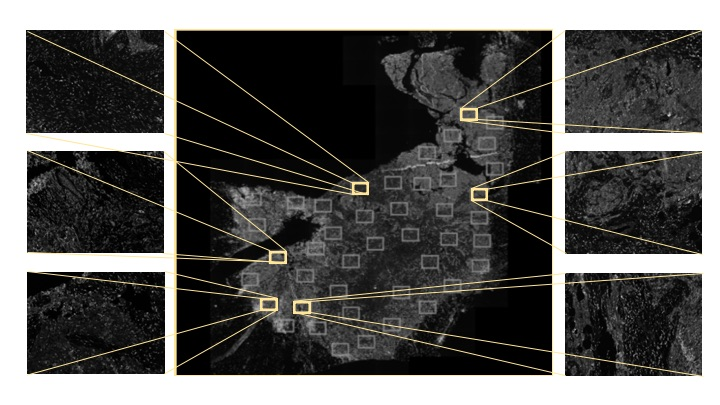
\includegraphics[width=\columnwidth]{doc/report/images/scan1.jpg}
  \caption{Example of a low resolution medical image with six high-resolution
snapshots. Middle: low-resolution of the whole slide with 45 snapshot positions
(small boxes). Left and Right: example of six high-resolution snapshots.}
  \vspace{-3mm}
  \label{fig:melanoma-scan}
\end{figure}


\section{State of the art}\label{sec:state-of-art}
\textbf{Survey the related work, giving credit where credit is
  due.} In the literature, several models have been proposed to perform super-resolution on medical images. We will survey them to get an idea what has already been done, from what we will take inspiration and what we decided to change. In ~\cite{zhang2019}, Zhang et al. propose a fast medical image super-resolution (FMISR) method with three hidden layers in addition to a sub-pixel convolution layer and a mini-network. This  model, they stipulate, improves image reconstruction speed and quality. Nevetheless, as it is used and trained on retinal macula, brain and bone images, it is not ideal for our stroma images, which are more cell oriented (\textbf{other way to formulate ?}). In ~\cite{nature2019}, Hongda Wang et al. present a deep-learning-enabled super-resolution across different fluorescence microscopy modalities. Their model is based on training a generative adversarial network (GAN) to create super resolution total internal reflection fluorescence (TIRF) microscopy images of sub-cellular structures from diffraction-limited input images. Nevertheless, we choose not to follow a GAN structure because of \textbf{TO COMPLETE}. In ~\cite{Janowczyk2018}, Janowczyk et al. introduce a resolution adaptive deep hierarchical (RADHicaL) learning scheme applied to nuclear segmentation of digital pathology images. In their model, "deep learning networks at lower resolutions are leveraged to determine if higher levels of magnification, and thus computation, are necessary to provide precise results"~\cite{Janowczyk2018}. While the images that are the focus of their report are much more similar to ours than the other state of the art methods, \textbf{TO complete why we don't want that}. 
  
  

\section{Models and Methods}\label{sec:models-methods}
\textbf{ Describe your idea and how it was implemented to solve
  the problem.}
The models and methods
section should describe what was
done to answer the research question, describe how it was done,
justify the experimental design, and
explain how the results were analyzed.

The model refers to the underlying mathematical model or structure which 
you use to describe your problem, or that your solution is based on. 
The methods on the other hand, are the algorithms used to solve the problem. 
In some cases, the suggested method directly solves the problem, without having it 
stated in terms of an underlying model. Generally though it is a better practice to have 
the model figured out and stated clearly, rather than presenting a method without specifying 
the model. In this case, the method can be more easily evaluated in the task of fitting 
the given data to the underlying model.

The methods part of this section, is not a step-by-step, directive,
protocol as you might see in your lab manual, but detailed enough such
that an interested reader can reproduce your
work~\cite{anderson04,wavelab}.

The methods section of a research paper provides the information by
which a study's validity is judged.
Therefore, it requires a clear and precise description of how an
experiment was done, and the rationale
for why specific experimental procedures were chosen.
It is usually helpful to
structure the methods section by~\cite{kallet04methods}:
\begin{enumerate}
\item Layout the model you used to describe the problem or the solution.
\item Describing the algorithms used in the study, briefly including
  details such as hyperparameter values (e.g. thresholds), and
  preprocessing steps (e.g. normalizing the data to have mean value of
  zero).
\item Explaining how the materials were prepared, for example the
  images used and their resolution.
\item Describing the research protocol, for example which examples
  were used for estimating the parameters (training) and which were
  used for computing performance.
\item Explaining how measurements were made and what
  calculations were performed. Do not reproduce the full source code in
  the paper, but explain the key steps.
\end{enumerate}
 

\section{Results}\label{sec:results}
\textbf{Show evidence to support your claims made in the
  introduction.}
  Organize the results section based on the sequence of table and
figures you include. Prepare the tables and figures as soon as all
the data are analyzed and arrange them in the sequence that best
presents your findings in a logical way. A good strategy is to note,
on a draft of each table or figure, the one or two key results you
want to address in the text portion of the results.

\section{Discussion}\label{sec:discussion}
  \textbf{Discuss the strengths and weaknesses of your
  approach, based on the results. Point out the implications of your
  novel idea on the application concerned.}
  
\section{Summary}\label{sec:summary}
  \textbf{Summarise your contributions in light of the new
  results.}

\section*{Acknowledgements}
TO COMPLETE.

\newpage
\bibliographystyle{IEEEtran}
\bibliography{literature}

\end{document}